%
% LaTeX template for the XLVI CILAMCE
%
\documentclass[a4paper,10pt]{book}
%%%%%%%%%%%%%%%%%%%%%%%%%%%%%%%%%%%%%%%%%%%%%%%%%%%%%%%%%%
% GRUMEC
%%%%%%%%%%%%%%%%%%%%%%%%%%%%%%%%%%%%%%%%%%%%%%%%%%%%%%%%%%
%Lagrangian position (inital configuration)
\newcommand{\lPosition}{\mathbf{x}}
\newcommand{\lPositionh}{\mathbf{x}^h} %Interpolated coordinate vector
\newcommand{\refPositionh}{\mathbf{x}_r^h} %Interpolated coordinate vector
\newcommand{\refPosition}{\mathbf{x}_r} %Interpolated coordinate vector
\newcommand{\lPositionComp}{x}
\newcommand{\lDomain}{\Omega_0} %Initial domain
\newcommand{\lBoundary}{\Gamma_0} %inital boundary
%Eulerian position (current configuration)
\newcommand{\ePosition}{\mathbf{y}}
\newcommand{\ePositionh}{\mathbf{y}^h}%Interpolated coordinate vector
\newcommand{\ePositionComp}{y}
\newcommand{\eDomain}{\Omega} %Current domain
\newcommand{\refDomain}{\Omega_r} %Current domain
\newcommand{\eBoundary}{\Gamma} %Current boundary
%Current velocity
\newcommand{\eVelocity}{\dot{\mathbf{y}}}
%Eulerian acceleration (current configuration) vector
\newcommand{\eAccel}{\ddot{\mathbf{y}}}
%rigth Cauchy-Green stretch tensor
\newcommand{\cauchyStretch}{\mathbf{C}}
%rigth Cauchy-Green stretch tensor
\newcommand{\cauchyStretchRef}{\mathbf{C}_r}
%Green-Lagrange strain tensor
\newcommand{\greenStrain}{\mathbf{E}}
\newcommand{\greenStrainRef}{\mathbf{E}_r}
%Second Piola-Kirchhoff Stress tensor
\newcommand{\sPiolaStress}{\mathbf{S}}
%First Piola-Kirchhoff Stress tensor
\newcommand{\fPiolaStress}{\mathbf{P}}
%Cauchy Stress tensonr
\newcommand{\cauchyStress}{\boldsymbol{\sigma}}
%Configuration change function
\newcommand{\cChange}{\mathbf{f}}
%Configuration change function from reference to current
\newcommand{\cChangeRef}{\mathbf{f}_r}
%Discrete Configuration change function from reference to current
\newcommand{\cChangeRefh}{\mathbf{f}^{h}_r}
%Gradient of Configuration change function
\newcommand{\cChangeGrad}{\mathbf{F}}
\newcommand{\cChangeRateGradRef}{{\dot{\cChangeGrad}}_r}
%Gradient of Configuration change function from reference domain
\newcommand{\cChangeGradRef}{{\cChangeGrad}_r}
%Discrete Gradient of Configuration change function from reference domain
\newcommand{\cChangeGradRefh}{{\cChangeGrad}^{h}_r}
%Gradient of Configuration change function from initial to reference domain
\newcommand{\cChangeGradx}{{\cChangeGrad}_{x}}
%Rate of congiguration change ref
\newcommand{\cChangeRateRef}{{\dot{\cChange}}_r}
%Mapping from parent to initial
\newcommand{\lMap}{{\cChange}^0}
%Mapping from parent to current
\newcommand{\eMap}{{\cChange}^1}
%Mapping from parent to ref
\newcommand{\refMap}{{\cChange}^1_r}
%Green-Lagrange strain rate tensor
\newcommand{\greenStrainRate}{\dot{\greenStrain}}
%reference Green-Lagrange strain rate tensor
\newcommand{\greenStrainRateRef}{{\dot{\greenStrain}}_r}
%rigth Cauchy-Green stretch tensor
\newcommand{\cauchyStretchh}{\mathbf{C}^h}
%Green-Lagrange strain tensor
\newcommand{\greenStrainh}{\mathbf{E}^h}
%Discretization configuration change function
\newcommand{\cChangeh}{\mathbf{f}^h}
%Discretization mapping function to initial
\newcommand{\mapInih}{\mathbf{f}^{0h}}
%Discretization mapṕing function to final
\newcommand{\mapFinh}{\mathbf{f}^{1h}}
%Gradient of Configuration change function
\newcommand{\cChangeGradh}{\mathbf{F}^h}
%Gradient of maping to current
\newcommand{\cChangeGradfh}{\pmb{\Phi}_{n+1}^{h}}
%Gradient of mapping to initial  - component
\newcommand{\cChangeGradihComp}{\left({\Phi}^{h}_r\right)}
%Gradient of mapping to current  - component
\newcommand{\cChangeGradfhComp}{\left({\Phi}^{h}_{n+1}\right)}
%Gradient of mapping to reference
\newcommand{\cChangeGradih}{\pmb{\Phi}_r^{h}}
%Maping to initial
\newcommand{\lMaph}{\mathbf{f}^{0h}}
%Maping to reference
\newcommand{\refMaph}{\pmb{\varphi}^{h}_r}
%Gradient of maping to initial
\newcommand{\eMaph}{\pmb{\varphi}^{h}_{n+1}}
%Green-Lagrange strain rate tensor
\newcommand{\greenStrainRateh}{\dot{\mathbf{E}}^h}
%Current spatially discrete velocity
\newcommand{\eVelocityh}{\dot{\mathbf{y}}^h}
%Eulerian acceleration (current configuration) vector
\newcommand{\eAccelh}{\ddot{\mathbf{y}}^h}
%Lagrangian Constitutive Tensor
\newcommand{\lagConst}{\mathbf{D}}
%Jacobian
\newcommand{\Jacobian}{J}
%reference Jacobian
\newcommand{\JacobianRef}{J_r}
%Discrete Jacobian
\newcommand{\Jh}{J^h}
%Gradient on lagrangian coordinates
\newcommand{\lGrad}{{\pmb{\nabla}}_{\mathbf{x}}}
%Gradient on reference coordinates
\newcommand{\refGrad}{\nabla_{\mathbf{x}_r}}
%Gradient on eulerian coordinates
\newcommand{\eGrad}{\nabla_{\mathbf{y}}}
%Push-foward operator
\newcommand{\pushf}{\chi}
%alphaGeneralized integrator
\newcommand{\integParf}{\alpha_f}
\newcommand{\integParm}{\alpha_m}
%spectral radius
\newcommand{\specRadius}{\rho_{\infty}}


%%%%%%%%%%%%%%%%%%%%%%%%%%%%%%%%%%%%%%%%%%%%%%%%%%%%%%%%%%
% TAFMS
%%%%%%%%%%%%%%%%%%%%%%%%%%%%%%%%%%%%%%%%%%%%%%%%%%%%%%%%%%
\newcommand{\density}{\rho}

\newcommand{\velocity}{\mathbf{u}}

\newcommand{\velocityD}{\mathbf{U}}

\newcommand{\velocityIND}{u}

\newcommand{\stress}{\sigma}

\newcommand{\sstresstensor}{\pmb{\sigma}}

\newcommand{\stresstensor}{\pmb{\sigma}}

%\newcommand{\dyadd}{\otimes}
\newcommand{\dyadd}{ }

\newcommand{\sgn}{\mathrm{sgn}}

\newcommand{\trace}{\mathrm{tr}}

\newcommand{\unittensor}{\mathbf{I}}

\newcommand{\increment}{\varDelta}

\newcommand{\imaginary}{\imath}

\newcommand{\complexspace}{{\mathbb C}}

\newcommand{\mdiffusivity}{\kappa}

\newcommand{\laplacian}{\Delta}

\newcommand{\viscosity}{\mu}

\newcommand{\kviscosity}{\nu}

\newcommand{\diffusivity}{\nu}

\newcommand{\strainrate}{\varepsilon}

\newcommand{\strainratetensor}{\pmb{\varepsilon}}

\newcommand{\snormal}{\mathbf{n}}

\newcommand{\normal}{\mathbf{n}}

\newcommand{\tangentialI}{\mathbf{t}_1}

\newcommand{\tangentialII}{\mathbf{t}_2}

\newcommand{\sbodyforce}{\mathbf{f}}

\newcommand{\externalforce}{\mathbf{f}}

\newcommand{\vzero}{\mathbf{0}}

\newcommand{\deriv}{\mathrm{d}}

\newcommand{\divergence}{\pmb{\nabla}}

\newcommand{\Reynolds}{\mathrm{Re}}

\newcommand{\Pe}{\mathrm{Pe}}

\newcommand{\straction}{\mathbf{h}}

\newcommand{\traction}{\mathbf{h}}

\newcommand{\tractionD}{\mathbf{H}}

\newcommand{\deformationgradient}{\mathbf{F}}


\newcommand{\disp}{\mathbf{y}}

\newcommand{\dispIND}{y}

\newcommand{\dispD}{\mathbf{Y}}

\newcommand{\vdisp}{\mathbf{w}}

\newcommand{\firstpiola}{\mathbf{P}}

\newcommand{\secondpiola}{\mathbf{S}}

\newcommand{\tangentStiffness}{\mathbf{D}}

\newcommand{\pos}{\mathbf{x}}

\newcommand{\matpos}{\mathbf{X}}

\newcommand{\sacce}{\mathbf{a}}

\newcommand{\sacceIND}{a}

\newcommand{\mpos}{\hat{\pos}}

\newcommand{\mdisp}{\hat{\disp}}

%\newcommand{\mvelocity}{\hat{\velocity}}
\newcommand{\mvelocity}{\mathbf{v}}

%\newcommand{\mvelocityD}{\hat{\velocityD}}
\newcommand{\mvelocityD}{\mathbf{V}}

%\newcommand{\mvelocityIND}{\hat{u}}
\newcommand{\mvelocityIND}{v}

\newcommand{\macce}{\hat{\sacce}}

\newcommand{\mdispD}{\hat{\dispD}}

\newcommand{\svelocity}{\mathbf{u}}

\newcommand{\svelocityIND}{u}

\newcommand{\sdiv}{\divergence}

\newcommand{\mdiv}{\divergence_{X}}

\newcommand{\mdivSymm}{\divergence_{X}^s}

\newcommand{\sdens}{\rho}

\newcommand{\mdens}{\rho_0}

\newcommand{\mnormal}{\hat{\mathbf{n}}}

\newcommand{\mtraction}{\hat{\mathbf{h}}}

\newcommand{\spress}{p}

\newcommand{\press}{p}

\newcommand{\pressD}{\mathbf{P}}

\newcommand{\elasticmoduli}{\varmathbb{C}}

\newcommand{\ielasticmoduli}{\mathbb{C}}

\newcommand{\mbulk}{\kappa}

\newcommand{\KPEN}{K_{\mathrm{PEN}}}

\newcommand{\nuPEN}{\nu_{\mathrm{PEN}}}

\newcommand{\smoduli}{\mu}

\newcommand{\vunknown}{\pmb{\phi}}

\newcommand{\sunknown}{\phi}

\newcommand{\sunknownD}{\pmb{\Phi}}

\newcommand{\stest}{w}

\newcommand{\vtest}{\mathbf{w}}

\newcommand{\utest}{\mathbf{w}}

\newcommand{\ptest}{q}

\newcommand{\Jb}{J_b}

\newcommand{\J}{J}

\newcommand{\solutions}{\mathcal{S}}

\newcommand{\weighting}{\mathcal{V}}

\newcommand{\ssolution}{\mathcal{S}_y}

\newcommand{\sweighting}{\mathcal{V}_y}

\newcommand{\usolution}{\mathcal{S}_u}

\newcommand{\phisolution}{\mathcal{S}_{\phi}}

\newcommand{\phiweighting}{\mathcal{V}_{\phi}}

\newcommand{\pweighting}{\mathcal{V}_p}

\newcommand{\psolution}{\mathcal{S}_p}

\newcommand{\uweighting}{\mathcal{V}_u}

\newcommand{\msolution}{\mathcal{S}_m}

\newcommand{\mweighting}{\mathcal{V}_m}

\newcommand{\solutionh}{\mathcal{S}^h}

\newcommand{\weightingh}{\mathcal{V}^h}

%parametric coordinate vector
\newcommand{\pcoordinate}{\pmb{\xi}}

\newcommand{\lagrangep}{\ell}

\newcommand{\force}{f}

\newcommand{\sunknownh}{\phi^h}

\newcommand{\stesth}{w^h}

\newcommand{\sctraction}{\mathrm{h}}

\newcommand{\sctractionh}{\mathrm{h}^h}

\newcommand{\vgiven}{\mathbf{g}}

\newcommand{\sgiven}{g}

\newcommand{\SUPS}{\tau_{\mathrm{SUPS}}}

\newcommand{\SUPG}{\tau_{\mathrm{SUPG}}}

\newcommand{\TAUCI}{C_I}

\newcommand{\PSPG}{\tau_{\mathrm{PSPG}}}

\newcommand{\SUGNi}{\tau_{\mathrm{SUGN1}}}

\newcommand{\SUGNii}{\tau_{\mathrm{SUGN2}}}

\newcommand{\SUGNiii}{\tau_{\mathrm{SUGN3}}}

\newcommand{\SUGNxii}{\tau_{\mathrm{SUGN12}}}

\newcommand{\LSIC}{\nu_{\mathrm{LSIC}}}

\newcommand{\LSICTCii}{\nu_{\mathrm{LSIC-TC2}}}

\newcommand{\LSICTGI}{\nu_{\mathrm{LSIC-TGI}}}

\newcommand{\LSICTGN}{\nu_{\mathrm{LSIC-HRGN}}}

\newcommand{\LSICLHC}{\nu_{\mathrm{LSIC-LHC}}}

\newcommand{\RGN}{h_{\mathrm{RGN}}}

\newcommand{\rRGN}{\mathbf{r}}

\newcommand{\tauTAN}{\tau_{\mathrm{TAN}}^B}

\newcommand{\tauNOR}{\tau_{\mathrm{NOR}}^B}

\newcommand{\TAUWBC}{\tau_\mathrm{B}}

\newcommand{\resMom}{\mathbf{r}_{\mathrm{M}}}

\newcommand{\resPre}{{r}_{\mathrm{C}}}

\newcommand{\resAD}{{r}_\mathrm{T}}

\newcommand{\forceh}{f^h}

\newcommand{\strainvector}{\pmb{\epsilon}}

\newcommand{\patom}{\press_{\mathrm{atm}}}

\newcommand{\pinfty}{\press_{\infty}}

\newcommand{\velocinfty}{\velocity_{\infty}}

\newcommand{\stressinfty}{\stresstensor_{\infty}}

\newcommand{\neb}{n_{\mathrm{eb}}}

\newcommand{\nel}{n_{\mathrm{el}}}

\newcommand{\ncp}{n_{\mathrm{np}}}

\newcommand{\nsd}{{n_{\mathrm{sd}}}}

\newcommand{\npd}{{n_{\mathrm{sd}}}}

\newcommand{\nc}{n_{\mathrm{c}}}

%\newcommand{\mc}{m_{\mathrm{c}}}

\newcommand{\lc}{l_{\mathrm{c}}}

\newcommand{\nk}{n_{\mathrm{k}}}

\newcommand{\mk}{m_{\mathrm{k}}}

\newcommand{\lk}{l_{\mathrm{k}}}

\newcommand{\realspace}{\mathbb{R}}

\newcommand{\nrealspace}{\mathbb{R}^{\nsd}}

\newcommand{\disph}{\mathbf{d}^h}

\newcommand{\vdisph}{\mathbf{w}^h}

\newcommand{\velocityh}{\mathbf{u}^h}

\newcommand{\sindexset}{\indexset^{s}}

\newcommand{\gindexset}{\indexset^{s}_\mathrm{g}}

\newcommand{\shapef}{N}

\newcommand{\shapet}{T}

\newcommand{\shaper}{R}

\newcommand{\testf}{Q}

\newcommand{\windexset}{\indexset^{w}}

\newcommand{\itercounter}{i}

\newcommand{\nen}{n_{\mathrm{en}}}

\newcommand{\nens}{n_{\mathrm{ens}}}

\newcommand{\nent}{n_{\mathrm{ent}}}

\newcommand{\indexset}{\pmb{\eta}}

\newcommand{\gsolutions}{u}

\newcommand{\gsolutiong}{g}

\newcommand{\gsolutionu}{v}

\newcommand{\gsolutionsh}{u^h}

\newcommand{\gsolutionsD}{\mathbf{U}}

\newcommand{\gsolutiongh}{g^h}

\newcommand{\gsolutionuh}{v^h}

\newcommand{\elementsize}{h}

\newcommand{\pressh}{p^h}

\newcommand{\Order}{\mathcal{O}}

\newcommand{\Jxxi}{J_{x\xi}}

\newcommand{\nint}{n_\mathrm{int}}

\newcommand{\nintt}{n_\mathrm{intt}}

\newcommand{\qiter}{\gamma}

\newcommand{\qweight}{w}

\newcommand{\domainST}{Q}

\newcommand{\domainSTn}{Q_n}

\newcommand{\domainSTE}{Q^e}

\newcommand{\domainSTnE}{Q_n^e}

\newcommand{\domainSTT}{Q_t}

\newcommand{\domainSTR}{\hat{Q}}

\newcommand{\domainSTTR}{Q_{\tilde{t}}}

\newcommand{\domainSTZE}{\hat{Q}^e}

\newcommand{\domainR}{\hat{\Omega}}

\newcommand{\domainRE}{\hat{\Omega}^e}

\newcommand{\domain}{\Omega}

\newcommand{\domainT}{\Omega_t}

\newcommand{\domainALEN}{\Omega_{t_{(n+\alpha_f)}}}

\newcommand{\domainN}{\Omega_n}

\newcommand{\domainNP}{\Omega_{n+1}}

\newcommand{\domainZ}{\Omega_0}

\newcommand{\domainTR}{\Omega_{\tilde{t}}}

\newcommand{\domainE}{\Omega^e}

\newcommand{\domainTE}{\Omega_t^e}

\newcommand{\boundary}{\Gamma}

\newcommand{\boundaryZ}{\Gamma_0}

\newcommand{\boundaryT}{\Gamma_{t}}

\newcommand{\boundaryH}{\Gamma_\mathrm{h}}

\newcommand{\boundaryZH}{\left(\Gamma_0\right)_\mathrm{h}}

\newcommand{\boundaryG}{\Gamma_\mathrm{g}}

\newcommand{\boundaryTG}{\left(\Gamma_t\right)_\mathrm{g}}

\newcommand{\boundaryB}{\Gamma^{b}}

\newcommand{\boundaryTH}{\left(\Gamma_t\right)_\mathrm{h}}

\newcommand{\boundaryST}{P}

\newcommand{\boundarySTn}{P_n}

\newcommand{\interfaceSTFSIn}{P_n}
\newcommand{\boundarySTFSIn}{P_n}

\newcommand{\boundarySTnH}{\left(P_n\right)_\mathrm{h}}

\newcommand{\boundarySTnG}{\left(P_n\right)_\mathrm{g}}

\newcommand{\domainFSI}{\Omega}

\newcommand{\domainFSIZ}{\Omega_0}

\newcommand{\domainFSIT}{\Omega_t}

\newcommand{\interfaceFSIZ}{\left(\Gamma_\mathrm{I}\right)_0}

\newcommand{\interfaceFSIT}{\Gamma_\mathrm{I}}

\newcommand{\interfaceFFSIT}{\Gamma_\mathrm{I1}}

\newcommand{\interfaceFFSINP}{\left(\Gamma_\mathrm{1I}\right)_{n+1}}

\newcommand{\interfaceFFSITT}{\left(\Gamma_\mathrm{1I}\right)_{\tilde{t}}}

\newcommand{\interfaceSFSIT}{\Gamma_\mathrm{2I}}
\newcommand{\interfaceSFSIZ}{(\Gamma_\mathrm{2I})_0}

\newcommand{\boundarySFSIT}{\Gamma_\mathrm{2E}}
\newcommand{\boundarySFSIZ}{(\Gamma_\mathrm{2E})_0}
\newcommand{\boundaryFFSIT}{\Gamma_\mathrm{1E}}
\newcommand{\boundaryFFSIZ}{(\Gamma_\mathrm{1E})_0}


\newcommand{\interfaceSFSINP}{\left(\Gamma_\mathrm{2I}\right)_{n+1}}

\newcommand{\interfaceFSIR}{\left(\Gamma_\mathrm{I}\right)_{\mathrm{REF}}}

\newcommand{\interfaceFFSIR}{\left(\Gamma_\mathrm{1I}\right)_{\mathrm{REF}}}

\newcommand{\interfaceSFSIR}{\left(\Gamma_\mathrm{2I}\right)_{\mathrm{REF}}}

\newcommand{\domainFSISTn}{Q_n}

\newcommand{\interfaceFSISTn}{\left(P_n\right)_\mathrm{h}}

\newcommand{\domainFluid}{\Omega_\mathrm{1}}

\newcommand{\domainFluidZ}{\left(\Omega_\mathrm{1}\right)_0}

\newcommand{\domainFluidT}{\left(\Omega_\mathrm{1}\right)_t}

\newcommand{\domainFluidN}{\left(\Omega_\mathrm{1}\right)_n}
\newcommand{\domainFluidNP}{\left(\Omega_\mathrm{1}\right)_{n+1}}

\newcommand{\domainFluidE}{\left(\Omega_\mathrm{1}\right)_t^e}

\newcommand{\interfaceFluidZH}{\left(\Gamma_\mathrm{1h}\right)_0}
\newcommand{\interfaceFluidTH}{\left(\Gamma_\mathrm{1h}\right)_t}
\newcommand{\interfaceFluidTG}{(\Gamma_\mathrm{1g})_t}
\newcommand{\interfaceFluidZG}{(\Gamma_\mathrm{1g})_0}
\newcommand{\interfaceFluidNPH}{\left(\Gamma_\mathrm{1h}\right)_{n+1}}

\newcommand{\domainFluidST}{Q}

\newcommand{\domainFluidSTn}{Q_n}

\newcommand{\domainFluidSTnE}{Q^e_n}

%\newcommand{\interfaceFluidSTnH}{\left(P_n\right)_\mathrm{h}}
\newcommand{\interfaceFluidSTnH}{P_n}

\newcommand{\domainStructure}{\Omega_\mathrm{2}}

\newcommand{\domainStructureZ}{\left(\Omega_\mathrm{2}\right)_0}
\newcommand{\domainStructureNP}{\left(\Omega_\mathrm{2}\right)_{n+1}}

\newcommand{\domainStructureT}{\left(\Omega_\mathrm{2}\right)_t}

\newcommand{\interfaceStructureTH}{(\Gamma_\mathrm{2h})_t}

\newcommand{\interfaceStructureZH}{\left(\Gamma_\mathrm{2h}\right)_{0}}
\newcommand{\interfaceStructureZG}{(\Gamma_\mathrm{2g})_{0}}
\newcommand{\interfaceStructureTG}{(\Gamma_\mathrm{2g})_{t}}

\newcommand{\domainMesh}{\left(\Omega_\mathrm{1}\right)_{\tilde{t}}}

\newcommand{\utestA}{\utest_\mathrm{1}}

\newcommand{\utestE}{\utest_\mathrm{1E}}

\newcommand{\ptestA}{\ptest_\mathrm{1}}

\newcommand{\ptestE}{\ptest_\mathrm{1E}}

\newcommand{\utestI}{\utest_\mathrm{1I}}

\newcommand{\ptestI}{\ptest_\mathrm{1I}}

\newcommand{\ptestII}{\ptest_\mathrm{2I}}

\newcommand{\mtest}{\mathbf{w}_\mathrm{3}}

\newcommand{\mtestE}{\mathbf{w}_\mathrm{3E}}

\newcommand{\mtestI}{\mathbf{w}_\mathrm{3I}}

\newcommand{\vdispA}{\mathbf{w}_\mathrm{2}}

\newcommand{\vdispI}{\mathbf{w}_\mathrm{2I}}

\newcommand{\vdispE}{\mathbf{w}_\mathrm{2E}}

\newcommand{\unknownDD}{\mathbf{d}}

\newcommand{\unknownF}{\mathbf{d}_\mathrm{1}}

\newcommand{\unknownS}{\mathbf{d}_\mathrm{2}}

\newcommand{\unknownM}{\mathbf{d}_\mathrm{3}}

\newcommand{\unknownFi}{\mathbf{d}_\mathrm{1}^i}

\newcommand{\unknownSi}{\mathbf{d}_\mathrm{2}^i}

\newcommand{\unknownMi}{\mathbf{d}_\mathrm{3}^i}

\newcommand{\unknownFii}{\mathbf{d}_\mathrm{1}^{i+1}}

\newcommand{\unknownSii}{\mathbf{d}_\mathrm{2}^{i+1}}

\newcommand{\unknownMii}{\mathbf{d}_\mathrm{3}^{i+1}}

\newcommand{\unknownGG}{\mathbf{u}}

\newcommand{\unknownFG}{\mathbf{u}_\mathrm{1}}

\newcommand{\unknownSG}{\mathbf{u}_\mathrm{2}}

\newcommand{\unknownMG}{\mathbf{u}_\mathrm{3}}

\newcommand{\unknownLL}{\mathbf{x}}

\newcommand{\unknownFL}{\mathbf{x}_\mathrm{1}}

\newcommand{\unknownSL}{\mathbf{x}_\mathrm{2}}

\newcommand{\unknownML}{\mathbf{x}_\mathrm{3}}

\newcommand{\unknownNN}{\mathbf{N}}

\newcommand{\unknownFN}{\mathbf{N}_\mathrm{1}}

\newcommand{\unknownSN}{\mathbf{N}_\mathrm{2}}

\newcommand{\unknownMN}{\mathbf{N}_\mathrm{3}}

\newcommand{\NNSM}{\mathbf{N}_\mathrm{M}}

\newcommand{\NNSC}{\mathbf{N}_\mathrm{C}}

\newcommand{\NNSMIND}{\mathrm{N}_\mathrm{M}}

\newcommand{\NNSCIND}{\mathrm{N}_\mathrm{C}}

\newcommand{\unknownRR}{\mathbf{b}}

\newcommand{\unknownFR}{\mathbf{b}_\mathrm{1}}

\newcommand{\unknownSR}{\mathbf{b}_\mathrm{2}}

\newcommand{\unknownMR}{\mathbf{b}_\mathrm{3}}

\newcommand{\unknownMM}{\mathbf{A}}

\newcommand{\unknownMP}{\mathbf{P}}

\newcommand{\unknownFZ}{\mathbf{z}_\mathrm{1}}

\newcommand{\unknownSZ}{\mathbf{z}_\mathrm{2}}

\newcommand{\unknownMZ}{\mathbf{z}_\mathrm{3}}

\newcommand{\dass}{\mathop{\mathlarger{\mathlarger{\sf A}}}_{e = 1}^{\nel}}

\newcommand{\NEVBeps}{\epsilon}

\newcommand{\nnp}{{n_n}}

\newcommand{\angularVelocity}{\pmb{\omega}}

\newcommand{\shellThickness}{h_\mathrm{th}}

\newcommand{\shellDomainZ}{\Gamma^s_0}

\newcommand{\shellDomainT}{\Gamma^s_t}

\newcommand{\bendingDomainZ}{\Gamma^b_0}

\newcommand{\shellDomainTH}{\left(\Gamma^s_t\right)_\mathrm{h}}

\newcommand{\shellDomainVZ}{\Omega_0}

\newcommand{\fluidTorque}{T_\mathrm{f}}

\newcommand{\TAFSM}{T{\raise0.3ex\hbox{\scriptsize $\bigstar$}}AFSM}

\newcommand{\curvature}{\kappa}

\newcommand{\curvatureTensor}{\pmb{\curvature}}

\newcommand{\workTotal}{W}

\newcommand{\workInternal}{W_{\mathrm{int}}}

\newcommand{\workExternal}{W_{\mathrm{ext}}}

\newcommand{\rotationTensor}{\mathbf{R}}

\newcommand{\rightStretchTensor}{\mathbf{U}}

\newcommand{\inflowBoundary}{\Gamma_\mathrm{IN}}

\newcommand{\meLUMP}{\mathbf{m}^e_\mathrm{LUMP}}

\newcommand{\ceHYFU}{C^e_\mathrm{ HYFU}}

\newcommand{\totalTime}{T}

\newcommand{\oneCardiacCycle}{T}

\newcommand{\interfaceOSI}{\left(\Gamma_\mathrm{1I}\right)_\mathrm{ROSI}}

\newcommand{\nInOutlets}{n_\mathrm{srf}}

\newcommand{\wallThickness}{h_{\mathrm{th}}}

\newcommand{\scafsiDisplacement}{\dispD}

\newcommand{\scafsiVelocity}{\mvelocityD}

\newcommand{\scafsiMeshDisplacement}{\mdispD}

\newcommand{\scafsiPress}{\pressD}

\newcommand{\scafsiStress}{\tractionD}

\newcommand{\nts}{n_\mathrm{ts}}

\newcommand{\wo}{\alpha}

\newcommand{\woim}{(\utestI^h)_{n+1}^-}

\newcommand{\woimsd}{\left(\utestI^h\right)}

\newcommand{\woimsdnopara}{\utestI^h}

\newcommand{\hvoi}{\left({\traction}^h_v\right)_\mathrm{1I}}

\newcommand{\tractionFE}{\traction_{\mathrm{1E}}}
\newcommand{\tractionSE}{\traction_{\mathrm{2E}}}
\newcommand{\tractionFI}{\traction_{\mathrm{1I}}}
\newcommand{\tractionSI}{\traction_{\mathrm{2I}}}

\newcommand{\poisonsRatio}{\nu}

\newcommand{\kporo}{k_\mathrm{PORO}}

\newcommand{\interfaceSlideT}{\left(\Gamma_t\right)_\mathrm{SI}}


% PACKAGES USED - packages that need to be previously installed on your computer
\usepackage[lmargin=2.5cm, rmargin=2.5cm, tmargin=2.5cm, bmargin=2.5cm ]{geometry}
\usepackage{graphicx}
\usepackage{times}
\usepackage{indentfirst}
\usepackage{fancyhdr}
\usepackage{titlesec}
\usepackage[english]{babel}
\usepackage{parskip} 
\usepackage{setspace}

\usepackage{amsmath}   % dá suporte a \begin{split}, align, etc.
\usepackage{amssymb}   % símbolos extras, \mathfrak, …
\usepackage{bm}        % comando \bm{…} para negrito em modo matemático

%%%%%%%%%%%%%%%%%%%%%%%%%%%%%%%%%%%%%%%%%%%%%%%%%%%%%%%%%%%%%%%%%
%%%%%%%%%%%%%%%%%%%%%%%%%%%%%%%%%%%%%%%%%%%%%%%%%%%%%%%%%%%%%%%%%
%%% My Additional Packages
%%%%%%%%%%%%%%%%%%%%%%%%%%%%%%%%%%%%%%%%%%%%%%%%%%%%%%%%%%%%%%%%%
\usepackage[utf8]{inputenc}
%\usepackage{amssymb} %Mathematics
%\usepackage{amsfonts}%Mathematics
%\usepackage{amsmath,amscd}%Mathematics
%\usepackage{amsthm}%Mathematics
%\usepackage{mathrsfs}%Mathematics font
%\usepackage{xspace}
%\usepackage{booktabs}
%\usepackage{stmaryrd}%Particular Brackets
%\usepackage{graphicx} %Tables and Figures
%\usepackage{subfigure}
%\usepackage{url}
\usepackage{hyperref}
\usepackage{cleveref}
\usepackage{./pkg-crefNames}
\usepackage[labelsep=period]{caption}

%BibTeX compatible with the CILAMCE format
\usepackage[numbers,sort&compress]{natbib}

\setlength{\bibsep}{0pt plus 0.3ex}

\renewcommand*{\bibfont}{\small}

\makeatletter
\renewcommand\bibsection
{
  \section*{References}
}

\renewenvironment{thebibliography}[1]
      {\section*{\refname}%
       \@mkboth{\MakeUppercase\refname}{\MakeUppercase\refname}%
       \list{\@biblabel{\@arabic\c@enumiv}}%
            {\settowidth\labelwidth{\@biblabel{#1}}%
             \leftmargin\labelwidth
             \advance\leftmargin-10pt% change 20 pt according to your needs
             \advance\leftmargin\labelsep
             \setlength\itemindent{10pt}% change using the inverse of the length used before
             \@openbib@code
             \usecounter{enumiv}%
             \let\p@enumiv\@empty
             \renewcommand\theenumiv{\@arabic\c@enumiv}}%
       \sloppy
       \clubpenalty4000
       \@clubpenalty \clubpenalty
       \widowpenalty4000%
       \sfcode`\.\@m}
      {\def\@noitemerr
        {\@latex@warning{Empty `thebibliography' environment}}%
       \endlist}
\renewcommand\newblock{\hskip .11em\@plus.33em\@minus.07em}
\makeatother

\makeatother
\bibliographystyle{./bib-cilamce}
%\bibliographystyle{plain}

%%%%%%%%%%%%%%%%%%%%%%%%%%%%%%%%%%%%%%%%%%%%%%%%%%%%%%%%%%%%%%%%%
%%%%%%%%%%%%%%%%%%%%%%%%%%%%%%%%%%%%%%%%%%%%%%%%%%%%%%%%%%%%%%%%%

% CONFIGURATION
\renewcommand*\arraystretch{1.5}
\renewcommand*\thesection{\arabic{section}}
%\hyphenpenalty=10000 % You can uncomment this to avoid hyphenization
\titleformat*{\section}{\large\bfseries}
\titleformat*{\subsection}{\bfseries}
\titlespacing\section{0pt}{20pt plus 2pt minus 2pt}{12pt plus 2pt minus 2pt}
\titlespacing\subsection{0pt}{20pt plus 0pt minus 0pt}{12pt plus 0pt minus 0pt}
\setlength{\parskip}{0pt} % Spacing between paragraphs
\setlength{\parindent}{0.75cm} % Paragraph identation
\setlength\abovecaptionskip{6pt}

% --------------------------------------------------------------------------
% DO NOT EDIT - SPECIAL HEADINGS OF XLIII CILAMCE
% --------------------------------------------------------------------------
\fancypagestyle{first}
{
\fancyhf{}
\fancyfoot[RO]{\footnotesize \textit{CILAMCE-2025 \\
Proceedings of the XLVI Ibero-Latin-American Congress on Computational Methods in Engineering, ABMEC\\
Vitória, Brazil, November 24-27, 2025}}
\renewcommand{\headrulewidth}{.0pt}
\renewcommand{\footrulewidth}{.5pt}
}

\pagestyle{fancy}
\fancyhf{}

\fancyfoot[LE]{\footnotesize \textit{CILAMCE-2025\\
Proceedings of the XLVI Ibero-Latin-American Congress on Computational Methods in Engineering, ABMEC\\
Vitória, Brazil, November 24-27, 2025}}

\fancyfoot[RO]{\footnotesize \textit{CILAMCE-2025\\
Proceedings of the XLVI Ibero-Latin-American Congress on Computational Methods in Engineering, ABMEC\\
Vitória, Brazil, November 24-27, 2025}}

\renewcommand{\headrulewidth}{.5pt}
\renewcommand{\footrulewidth}{.5pt}

% --------------------------------------------------------------------------
% PLEASE, EDIT THIS!
\fancyhead[LE]{\footnotesize \textit{Template file for CILAMCE-2025 full-length paper (enter here with the short title of your paper)}}
\fancyhead[RO]{\footnotesize \textit{F. Author, S. Author, T. Author}}
% --------------------------------------------------------------------------

\begin{document}\thispagestyle{first}

% --------------------------------------------------------------------------
% DO NOT EDIT - LOGO OF XLIII CILAMCE
% --------------------------------------------------------------------------

\begin{figure}[ht!]
\vspace{-30pt}
\flushright
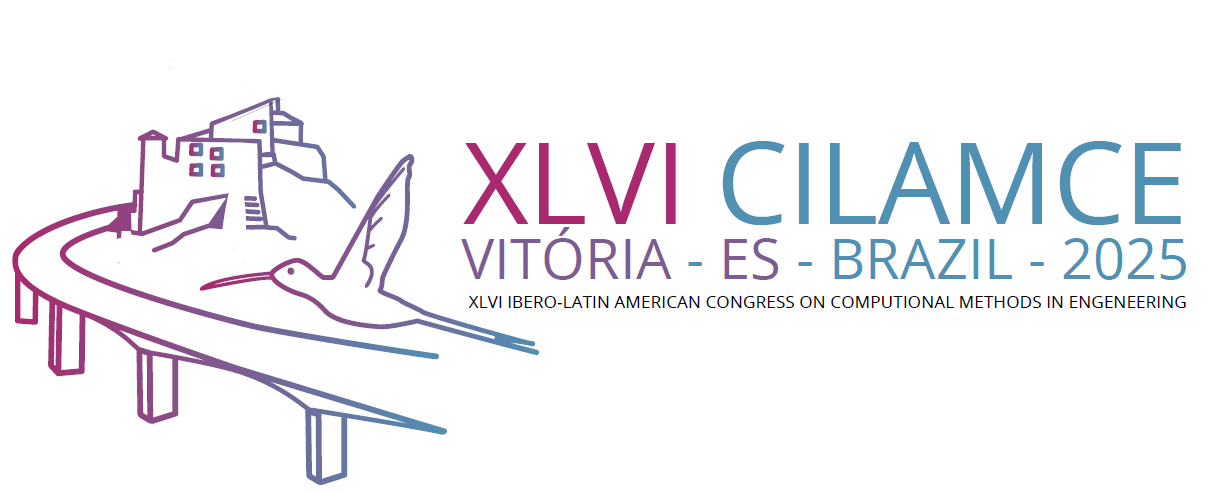
\includegraphics[width=6.69cm]{Figures/logo.png}
%scale=0.25
\end{figure}

% --------------------------------------------------------------------------
% TITLE OF PAPER
% --------------------------------------------------------------------------

\noindent
\textbf{\Large
A Monolithic Framework for the Simulation of Free-Surface Non-Newtonian Fluid Flow with Multiple Immersed Elastic Solids} 
\vspace{18pt} % <- keep this vertical space!

% --------------------------------------------------------------------------
% AUTHORS
% --------------------------------------------------------------------------

\noindent Luiz Fernando Honorato Teodoro$^1$, Rodolfo André Kuche Sanches$^1$

\vspace{18pt} % <- keep this vertical space!

\noindent $^1$\textit{Structural Engineering Department, S\~ao Carlos School of Engineering, University of S\~ao Paulo}

\noindent \textit{Av. Trabalhador Saocarlense, 400, S\~ao Carlos, S\~ao Paulo, Brazil}

\noindent \textit{luizteodoro@usp.br, rodolfo.sanches@usp.br}


\vspace{18pt} % <- keep this vertical space!

% --------------------------------------------------------------------------
% ABSTRACT
% --------------------------------------------------------------------------

  \noindent \textbf{Abstract.}
  This work presents a monolithic computational framework for simulating free-surface incompressible non-Newtonian flows with multiple immersed solid bodies. The methodology combines a particle-position-based formulation of the Particle Finite Element Method (PFEM) for the fluid phase and a total Lagrangian finite element formulation for the solid phase. Both fluid and solid models use nodal positions as primary variables. This unified treatment enables direct and consistent coupling between fluid and solid domains. Interactions between immersed solids are handled through a node-to-surface contact formulation enforced via Lagrange multipliers. The fluid is described by the Herschel-Bulkley-Papanastasiou (HBP) constitutive model, while the solid is described by the Saint-Venant-Kirchhoff (SVK) constitutive model. For temporal discretization, the implicit Generalized-$\alpha$ time-marching scheme is adopted, offering second-order accuracy and enhanced stability through controlled numerical dissipation of high-frequency effects. The proposed methodology demonstrates strong potential for applications such as simulating concrete flow, where the mortar is treated as a non-Newtonian fluid and the coarse aggregates as immersed solid particles.



\vspace{18pt} % <- keep this vertical space!

\noindent \textbf{Keywords:} PFEM; free-surface flow; non-Newtonian fluid; immersed solids; FSI.


% --------------------------------------------------------------------------
\section{Introduction}\label{sec:introduction}
% --------------------------------------------------------------------------

  Modeling multiple immersed solid bodies within a fluid domain is a significant challenge in computational mechanics, as it typically involves the simultaneous treatment of fluid-solid interaction (FSI), solid contact, and, in most cases, free-surface flow. To address such problems, \citet{Onate2014} employed a combination of the Particle Finite Element Method (PFEM) — well suited for flows with topological changes — to model the fluid domain, together with the Finite Element Method (FEM) and the Discrete Element Method (DEM) for the solid domain. These authors presented various problems, such as landslides impacting houses and the dragging of rocks by a water stream.

  \citet{Idelsohn2004} introduced a hybrid approach known as PFEM, which combines the advantages of particle-based methods with the robustness of mesh-based techniques. This methodology uses particles to represent the fluid domain, which are then employed to generate a finite element mesh for solving the governing equations, with periodic remeshing to maintain mesh quality throughout the simulation.

  Building upon this method, \citet{Avancini2024} proposed a particle-position-based PFEM formulation for simulating free-surface incompressible Newtonian flows, using nodal positions and pressures as the primary unknowns instead of the more common velocities and pressures. This choice naturally incorporates geometric nonlinearities, eliminates the need for a separate step to compute displacements from nodal velocities, and is well suited for monolithic coupling of fluid and solid phases. Subsequently, \citet{Teodoro2024} extended this framework to incompressible non-Newtonian fluids, specifically for the Bingham-Papanastasiou model, demonstrating its effectiveness in fresh concrete flow simulations.

  In this context, the present work builds upon this approach by adopting a more complete constitutive model and incorporating multiple immersed solid bodies. The HBP model is employed to describe the fluid phase, which is more suitable for simulating materials with non-linearity after the yield stress, such as fresh concrete. The solid phase is described by the SVK constitutive model, allowing for large displacements. The interaction between immersed solids is handled through a node-to-surface contact formulation enforced via Lagrange multipliers, allowing for accurate representation of contact forces and preventing interpenetration. The coupling between the fluid and solid phases is achieved through a monolithic approach.

% --------------------------------------------------------------------------
\section{Continuum mechanics}\label{sec:continuumMechanics}
% --------------------------------------------------------------------------

  We briefly describe the kinematic measures, governing equations, and constitutive models for the fluid and solid domains.

  % --------------------------------------------------------------------------
  \subsection{Kinematic measures and governing equations}\label{subsec:kinematicMeasures}
  % --------------------------------------------------------------------------
  
    In the total Lagrangian description adopted for the solid, the reference configuration is always the initial $\Omega_0$. For the fluid, due to the recurrent remeshing in PFEM, the reference configuration $\Omega_r$ corresponds to the state at the instant preceding the current time step $t_{n+1}$, representing a partially updated Lagrangian description. In this section, all equations are written with variables carrying the subscript $r$, but interpreted according to each domain's own reference configuration.

    The reference and current configurations are represented by the coordinates $\refPosition$ and $\ePosition$, respectively, and the deformation gradient tensor $\cChangeGradRef$ is then defined as:
    \begin{equation} \label{eq:defGrad} 
      \cChangeGradRef = \refGrad \ePosition
    \end{equation}

    The governing equations are momentum and mass conservation. The latter can be expressed in terms of the Jacobian determinant ($J_r = \left| \cChangeGradRef \right|$), which represents the volumetric change of an infinitesimal element relative to its reference volume. For an incompressible fluid, the Jacobian is constant in time and equal to one. Therefore, in the reference configuration these equations can be written as:
    \begin{equation} \label{eq:MomentumLocal}
      \rho \ddot{\mathbf{y}} - \refGrad \cdot
      \left(\mathbf{S}\cChangeGradRef^T \right) - \mathbf{b}_r = \mathbf{0} 
    \end{equation}
    \begin{equation}\label{eq:Incompsolid}
      \JacobianRef = \frac{\rho_r}{\rho}
    \end{equation}
    where $\rho$ is the fluid density, $\eAccel$ is the material derivative of the fluid velocity, $\mathbf{S}$ is the second Piola-Kirchhoff stress tensor, and $\mathbf{b}_r$ is the body force vector.

    These equations are complemented by the boundary conditions, expressed as:
    % \vspace{6pt}
    % \begin{center}    
    \begin{equation} \label{eq:Dirichlet}
          \mathbf{y} = \mathbf{y}_D \text{ on } \Gamma_D 
        \end{equation}
    % \end{center}
    %     \vspace{6pt}
    %     \vspace{6pt}
    %     \begin{center}
        \begin{equation} \label{eq:Neumann}
          \left(\mathbf{S}\cChangeGradRef^T\right)\mathbf{n}_r = \mathbf{h}_r \text{ on } \Gamma_N 
        \end{equation}
    % \end{center}
    % \vspace{6pt}
    where $\ePosition_D$ are the positions prescribed at the Dirichlet boundary ($\Gamma_D$), $\mathbf{h}_r$ are the tractions precribed at the Neumann boundary ($\Gamma_N$), and $\mathbf{n}_r$ is the normal vector to $\Gamma_N$.

  % --------------------------------------------------------------------------
  \subsection{Constitutive models}\label{subsec:constitutiveModels}
  % --------------------------------------------------------------------------

    We adopt the SVK model for the solid phase, a hyperelastic formulation expressed in the stress-strain relation as:
      \begin{equation}\label{eq:stressStrainSolid}
          \sPiolaStress = \mathbf{\mathfrak{C}} : \greenStrain_r \text{,}
      \end{equation}
      with
        \begin{equation}\label{eq:constitutiveSolid}
              \mathfrak{C} = \lambda \mathbf{I} \otimes \mathbf{I} + 2 G \mathbf{II}_s \text{,}
        \end{equation}  
      and
      \begin{equation}
          \mathbf{E}_r = \frac{1}{2} \left( \mathbf{C}_r - \mathbf{I} \right),
      \end{equation}
    where $\mathbf{\mathfrak{C}}$ is the fourth-order constitutive tensor, $\lambda$ and $G$ are the Lamé coefficients, $\mathbf{I}$ is the identity tensor, $\mathbf{II}_s$ is the second-order identity tensor, $\greenStrain$ is the Green-Lagrange strain tensor, and $\mathbf{C}_r = \cChangeGrad^T_r \, \cChangeGrad_r$ is the right Cauchy-Green deformation tensor.

    For the fluid phase, we choose the HBP model. First, the model is expressed through the Cauchy stress in the current configuration $\Omega$ as:
    \begin{equation} \label{eq:cauchyStress} 
        \cauchyStress = \boldsymbol{\tau} - \press \mathbf{I}  
    \end{equation}
    where $\boldsymbol{\tau}$ is the deviatoric stress tensor, $p$ is the pressure.

    The Herschel-Bulkley model includes three experimental parameters: the consistency index $k$, the yield stress $\tau_0$, and the flow behavior index $o$. To avoid numerical difficulties, we adopt the regularization proposed by \citet{Papanastasiou1987}, introducing a regularization parameter $m$. The deviatoric stress tensor is then given by:
    \begin{equation} \label{eq:HBP}
      \boldsymbol{\tau} = 2\left( k \left\| \dot{\boldsymbol{\varepsilon}} \right\|^{o-1} + \frac{\tau_0}{\left\| \dot{\boldsymbol{\varepsilon}} \right\|} \left( 1 - e^{-m \left\| \dot{\boldsymbol{\varepsilon}} \right\|} \right) \right) \boldsymbol{\dot{\varepsilon}} \text{,}
    \end{equation}
    where $\left \| \dot{\boldsymbol{\varepsilon}} \right \|$ is the equivalent strain rate, calculated as
    \begin{equation} \label{eq:equivalentStrainRate} 
      \left \| \dot{\boldsymbol{\varepsilon}} \right \| = \sqrt{2\dot{\boldsymbol{\varepsilon}}:\dot{\boldsymbol{\varepsilon}}} \text{,}
    \end{equation}
    and the strain rate tensor is
    \begin{equation} \label{eq:strainRate} 
      \dot{\boldsymbol{\varepsilon }}=\frac{1}{2}
      \left(\eGrad^T{\dot{\ePosition}}+\eGrad{\dot{\ePosition}}\right) \text{.}
    \end{equation}

    The deviatoric stress tensor can be written as the double contraction between an Eulerian constitutive tensor and the Eulerian strain rate tensor:
    \begin{equation} \label{eq:deviatoric}
        \boldsymbol{\tau} = \bm{\mathfrak{D}} : \dot{\boldsymbol{\varepsilon}} \text{,}
    \end{equation}
    where $\bm{\mathfrak{D}}$ is a fourth-order constitutive tensor, whose components are:
    \begin{equation} 
        D_{ijkl} = \left( k \left\| \dot{\boldsymbol{\varepsilon}} \right\|^{n-1} + \frac{\tau_0}{\left\| \dot{\boldsymbol{\varepsilon}} \right\|} \left( 1 - e^{-m \left\| \dot{\boldsymbol{\varepsilon}} \right\|} \right) \right) \left( \delta_{ik} \delta_{jl} + \delta_{il} \delta_{jk} \right) \text{,}
    \end{equation}
    with $\delta$ denoting the Kronecker delta.  
    This constitutive tensor is defined in the current configuration, and a pull-back operation is required to express it in the reference configuration due to the Lagrangian descriptions of the domains. Thus, the \eqref{eq:cauchyStress} becomes:
    \begin{equation} \label{eq:constitutiveTensorFluid}
        \sPiolaStress = \bm{\mathfrak{D}}_r : \greenStrainRateRef - \press \JacobianRef \cauchyStretchRef^{-1} \text{,}
    \end{equation}
    with 
    \begin{equation} \label{eq:E-rate}
        \greenStrainRateRef = \frac{1}{2} \left( \cChangeRateGradRef^T \cChangeGradRef + \cChangeGradRef^T \cChangeRateGradRef \right) \text{,}
    \end{equation}
    and
    \begin{equation} \label{eq:tensor-constitutive-reference} 
        (D_r)_{ijkl} = \JacobianRef \left(F_r^{-1}\right)_{ia} \left(F_r^{-1}\right)_{jb} \left(F_r^{-1}\right)_{kc} \left(F_r^{-1}\right)_{ld} D_{abcd}  \text{,}
    \end{equation}
    where $\greenStrainRateRef$ is the rate of the Green-Lagrange strain tensor, and $\cChangeRateGradRef$ is the rate of the deformation gradient.


% --------------------------------------------------------------------------
\section{Numerical strategies}\label{sec:numericalStrategies}
% --------------------------------------------------------------------------

  Regarding the spatial discretization of the continuum, both fluid and solid domains are discretized using linear finite elements (triangles in 2D and tetrahedra in 3D). The unknowns are approximated by nodal values and Lagrange polynomials with linear interpolation. Moreover, in the fluid domain, the pressure is also discretized using linear finite elements. For the temporal discretization, we employ the Generalized-$\alpha$ method proposed by \citet{Chung1993}, which is implicit, second-order accurate, unconditionally stable, and allows control of numerical dissipation at high frequencies. The equilibrium is evaluated at an intermediate time $t_{n+\alpha}$. 

% -------------------------------------------------------------------------
\subsection{Position-based finite element method for elastic solids} \label{subsec:MEFposicional}

% --------------------------------------------------------------------------

  The equilibrium equations for solid dynamics are obtained from the stationary energy principle taking the nodal positions and are given by:
  \begin{equation} \label{eq:full-solid-discretization}
    \frac{\partial{\Pi_{n+\alpha}}}{\partial (\ePosition_a)_{n+\alpha}} = 
    \int_{\Omega_0} \rho_0 N_a \eAccelh_{n+\alpha} d\Omega_0 +
    \int_{\Omega_0} \sPiolaStress^h_{n+\alpha} : \frac{\partial{(\greenStrain^h)_{n+\alpha}}}{\partial(\ePosition_a)_{n+\alpha}} d\Omega_0 - \int_{\Omega_0} N_a\mathbf{b}_{0} d\Omega_0 - 
    \int_{\Gamma_{0}}N_a\mathbf{h}_{0} d\Gamma_{0} = \mathbf{0} ,
  \end{equation}
  where $\Pi_{n+\alpha}$ is the total mechanical energy functional and $\mathbf{h}_0$ are the surface forces in the initial configuration. The supercript $h$ indicates that the variable is approximated by finite elements, the subscipt $a$ denotes the node, and the subscript $n+\alpha$ indicates that the variable is evaluated at the intermediate time $t_{n+\alpha}$.

% --------------------------------------------------------------------------
\subsection{Particle-position-based PFEM formulation} \label{subsec:PFEM}
% --------------------------------------------------------------------------

  In the work of \citet{Avancini2024}, the authors present the details of the particle-position-based PFEM formulation, which will be omitted here. As with the solid phase, the equilibrium equations for the fluid phase are obtained from the stationary energy principle, but in this case, the nodal positions and pressures are the unknowns. Applying this principle taking the nodal positions, we obtain:
  \begin{equation} \label{eq:fluidMomentum}
      \begin{split}
          &\frac{\partial{\Pi_{n+\alpha}}}{\partial (\ePosition_a)_{n+\alpha}} =
          \int_{\Omega_r} \rho_r N_a \eAccelh_{n+\alpha} d\Omega_r +
          \int_{\Omega_r} (\greenStrainRate_r^h)_{n+\alpha} : (\bm{\mathfrak{D}}^h_{r})_{n+\alpha} : \frac{\partial{(\greenStrain_r^h)_{n+\alpha}}}{\partial(\ePosition_a)_{n+\alpha}} d\Omega_r \\&-
          \int_{\Omega_r} p_{n+1}^h (J_r^h)_{n+\alpha} \, (\mathbf{C}_r^h)_{n+\alpha}^{-1} : 
  \frac{\partial (\mathbf{E}_r^h)_{n+\alpha}}{\partial (\mathbf{y}_a)_{n+\alpha}} d\Omega_r - \int_{\Omega_r} N_a\mathbf{b}_{r} d\Omega_r - 
          \int_{\Gamma_{r}}N_a\mathbf{h}_{r} d\Gamma_{r} = \mathbf{0} ,
      \end{split}
  \end{equation}
  where the first term on the right-hand side represents the inertial nodal force, the second and third terms correspond to the viscous and pressure parts of the internal nodal force, and the last terms represent the external nodal force. 

  Applying the principle of stationary energy with respect to the nodal pressures and adding the stabilization term, we obtain the discrete form of the incompressibility (or continuity) equation:
  \begin{equation} \label{eq:fluidContinuity}
      \begin{split} 
          \frac{\partial{\Pi_{n+\alpha}}}{\partial (p_a)_{n+1}} + \left((R_s)_a\right)_{n+\alpha} = &
          -\int_{\Omega_r} \shapef_a((\Jh_r)_{n+\alpha}-1) d\Omega_r + \int_{\Omega_{r}} \PSPG \frac{1}{\density_r} (\cChangeGrad_r^{h})^{-T}_{n+\alpha}\nabla_{\mathbf{x}_r} \shapef_a \cdot\biggl[\\& \quad\qquad
          \rho_r \eAccelh_{n+\alpha} -\nabla_{\mathbf{x}_r} \cdot
          \left((\mathbf{S}^h)_{n+\alpha}(\cChangeGrad^{h}_r)^T_{n+\alpha} \right) -\mathbf{b}_r \biggr]
          d\Omega_r = 0 \text{,}
      \end{split}
  \end{equation}
  where $\left((R_s)_{n+\alpha}\right)_a$ represents the contribution of the stabilization term to node $a$, and $\PSPG$ is a stabilization parameter. The nonlinear system defined by \cref{eq:fluidMomentum} and \cref{eq:fluidContinuity} is solved iteratively using the Newton-Raphson method.

  Due to the mandatory use of linear shape functions for both positions and pressure in PFEM, the Ladyzhenskaya-Babuška-Brezzi (LBB) conditions \citep{Babuska1973, Brezzi1974, BABUSKA1997183} are not satisfied. This can lead to spurious pressure solutions and numerical instability. To address this issue, the formulation employs the Pressure-Stabilized Petrov-Galerkin (PSPG) method \citep{tezduyar1991, TEZDUYAR1992221}, which consists of adding to the weak form the residual of the momentum equation, weighted by the gradient of the pressure test function and multiplied by a stabilization parameter.

  \citet{Cremonesi2020} and \citet{Avancini2024} provide an in-depth description of the PFEM technique. Here, we highlight the main steps of the method:
  \vspace{6pt}
    \begin{itemize}
      \item Filling the fluid domain with particles containing physical and kinematic properties;
      \item Generating a finite element mesh using Delaunay triangulation, where particles serve as nodes;
      \item Defining the domain boundaries using the $\alpha$-shape technique, as described by \citet{Edelsbrunner1994};
      \item Deforming the domain following equilibrium;
      \item Destroying the mesh when significant distortions occur, leaving only the particles.
    \end{itemize}
  \vspace{6pt}

  In the present work, this procedure is cyclic and repeats at each time step, without checking whether it is necessary to destroy the current discretization. We use GMSH to generate the initial finite element mesh and employ the open-source library TETGEN \citep{Si2015} for remeshing.


% --------------------------------------------------------------------------
\subsection{Solid-solid contact: node-to-surface formulation}\label{subsec:solidSolidContact}
% --------------------------------------------------------------------------

  The solid-solid contact formulation proposed in this work comprises two main steps: contact detection via a node-to-surface technique and enforcement of the contact constraints using Lagrange multipliers. 

  In the first step, it is necessary to define potential contact pairs, each consisting of one projectile node and a target surface. Each projectile node is represented solely by its position vector $\mathbf{y}_N$, while the points $\mathbf{y}_S$ on the target surface are obtained by interpolating the nodal coordinates of its element. To detect contact, these positions are also interpolated in dimensionless time. Contact occurs when the projectile trajectory intersects the target surface trajectory, determined by solving the nonlinear equation
  \begin{equation}
  \mathbf{r}(\omega, \boldsymbol{\xi}) = \mathbf{y}_N^{t}(\omega) - \mathbf{y}_S^{t}(\omega, \boldsymbol{\xi}) = \mathbf{0} \text{,}
  \end{equation}
  where $\omega$ is the time parameter ($0$ for the previous step and $1$ for the current), and $\boldsymbol{\xi}$ is the dimensionless coordinate of the target surface element. The solution of this equation is obtained using Newton's method, and after convergence it is verified whether $\boldsymbol{\xi}$ belongs to the target surface element and $\omega$ lies within $[0,1]$, activating the contact pair if both conditions are satisfied.

  In the second step, a Lagrange multiplier $\lambda_N$ is introduced for each contact pair to represent the activated contact force, thereby increasing the number of degrees of freedom in the system. The contact constraint is imposed by adding the following term to the energy functional:
  \begin{equation}
  \Pi_\text{c} = \lambda_N g_n = \lambda_N \left[ (\mathbf{y}_N - \mathbf{y}_S(\boldsymbol{\xi})) \cdot \mathbf{\bar{n}}(\boldsymbol{\xi}) \right],
  \end{equation}
  where $g_n$ measures the projected distance between the projectile node and the contact point on the target element, and $\mathbf{\bar{n}}(\boldsymbol{\xi})$ is the unit normal vector to the target surface at that point.  

  The principle of stationary energy is then applied with respect to the Lagrange multipliers, the projectile node, and the target surface nodes, adding the corresponding contributions to the solid equilibrium equations \eqref{eq:full-solid-discretization}. A contact pair is deactivated when the contact force exceeds the adhesion force and is positive, thereby reducing the number of DOFs in the system. Both steps are performed at each time step after updating the solid positions, and when there is a change of contact state, the Newton-Raphson procedure is restarted before proceeding to the next time step.

  In the present work, due to the large number of solid bodies, additional techniques are required to make the computational cost viable. Since each body contains many nodes and surface elements, assigning all nodes as potential projectiles for all surfaces would be unfeasible. To address this, a two-layer search strategy is employed.

  In the first layer, neighboring inclusions are identified by enclosing all solid bodies within a bounding box, allowing each node to be assigned an inclusion tag. In the second layer, a container is filled for each node with nearby target elements. This is achieved by subdividing the bounding box into smaller cells and using the neighboring inclusion information to restrict the search to relevant elements.

  Additionally, the generation and distribution of multiple solid bodies within the fluid domain follow the algorithm proposed by \citet{Wriggers2006}. This procedure comprises two stages: (i) solid generation, considering random mesoscopic geometries, and (ii) random and uniform placement within the domain. For this purpose, Wriggers and Moftah (2006) proposed the take-and-place method, in which solids are positioned one by one at random coordinates, ensuring no overlap and full containment within the domain.

\subsection{Monolithic coupling for fluid-solid interaction}\label{subsec:fsi}
% --------------------------------------------------------------------------

  In the monolithic coupling for FSI, the motions of the fluid and solid are solved in an integrated manner within a single system. The interaction is enforced through the contributions of both domains at the interface nodes. During the pre-processing stage, it is necessary to mark the potential interface nodes so that, after the intrinsic remeshing of the PFEM, interaction can occur if the fluid and solid come into proximity during the simulation.

% --------------------------------------------------------------------------
\section{Numerical results}\label{sec:numericalResults}
% --------------------------------------------------------------------------

  In \citet{Teodoro2024}, the formulation for Bingham-Papanastasiou fluid was validated using experimental and numerical data from the literature. Since the implementation of the HBP model is similar, we present here only a analytical verification by simulating a well-known benchmark: the Poiseuille flow. The configuration parameters are: channel height $h = 0.02 \ \text{m}$, density $\rho = 1000.0 \ \text{kg/m}^3$, consistency index $K = 10.0 \ \text{Pa$\cdot$s}$, regularization parameter $1000.0$, body force (in the horizontal direction) $b_1 = 20000 \ \text{N/m}^3$, element characteristic length $h_e = 0.0005 \ \text{m}$, tolerance $10^{-6}$, number of steps $2000$, and time step $\Delta t = 0.00005 \ \text{s}$. Figure \ref{poiseuille} shows the good agreement between the analytical solution and the numerical results.
  \begin{figure}[!ht]
  \begin{center}
  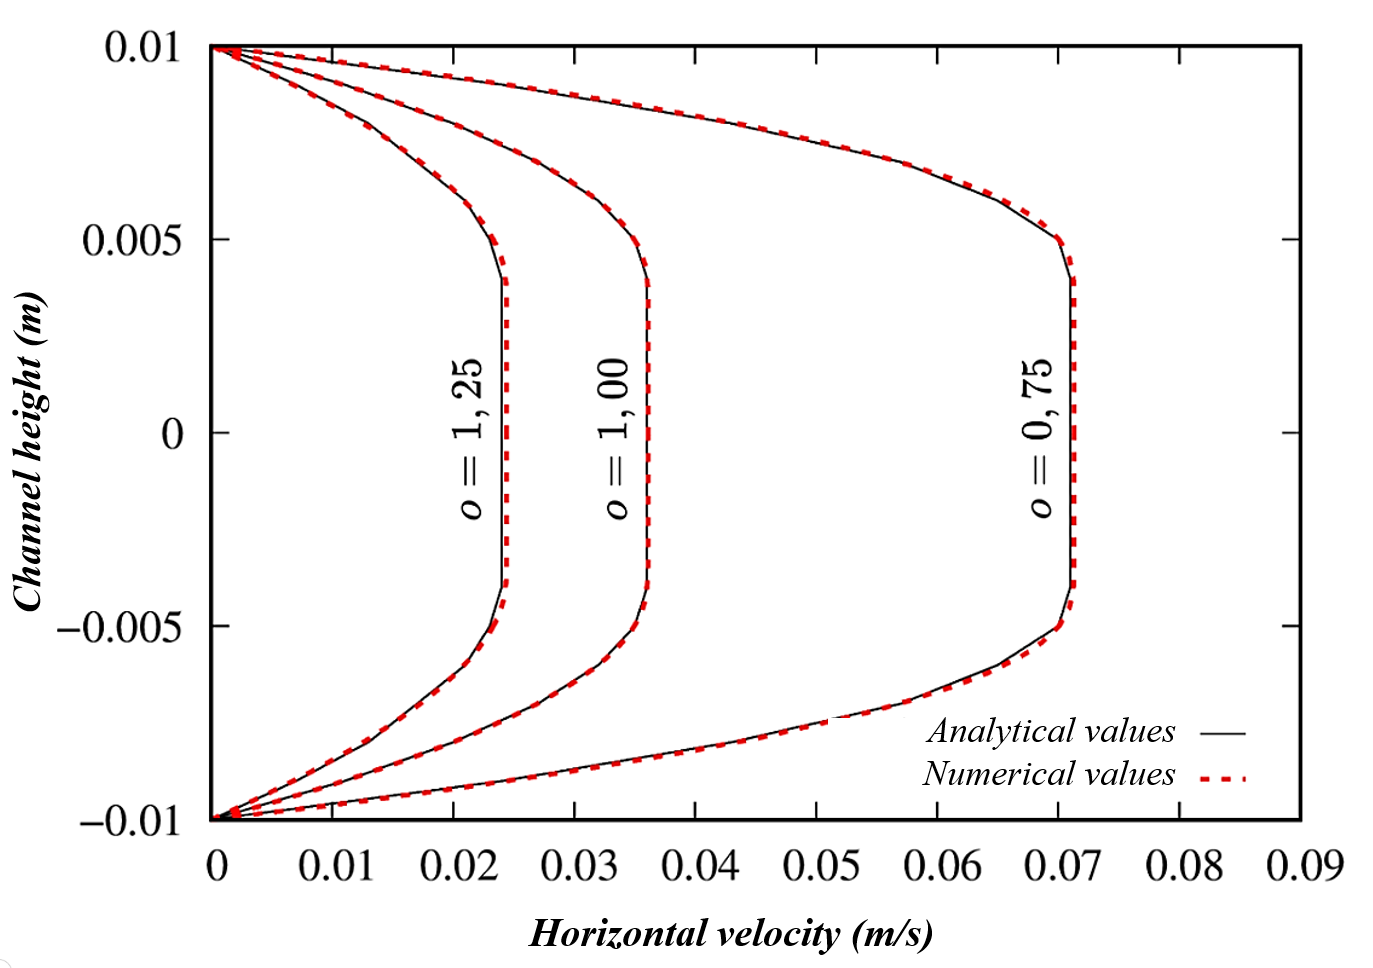
\includegraphics[scale=0.3]{Figures/poiseuille.png}
  \caption{Analytical and numerical velocity profiles for a Poiseuille flow varying flow behavior index}
  \label{poiseuille}
  \end{center}
  \end{figure}
  % \vspace{8pt}

  To verify the implementation of the contact algorithm, we simulate a benchmark consisting of the impact between two identical bars, each with a length of $25.4$ cm, moving towards each other with the same velocity. The bars have an initial gap of $0.0508$ cm, Young's modulus $E = 2.068 \ \text{MN/cm}^2$, density $\rho = 7.93 \times 10^{-6} \ \text{kg·s}^2/\text{cm}^4$, and a characteristic element size of $h_e = 0.30$ cm. The time step is set to $\Delta t = 1.0 \times 10^{-6}$ s, the number of steps to $210$, and the nonlinear tolerance to $10^{-6}$.  

  The analytical solution corresponds to a constant compressive stress wave propagating along the bar at speed $c = \sqrt{E/\rho}$, with magnitude $\sigma_{11} = \rho v_1 c$. The contact time is given by $t_{\text{contact}} = 2 \times 25.4 / 510668 \approx 10^{-4}$ s, after which separation occurs. Figure~\ref{contactVerification} compares the analytical and numerical Cauchy stress $\sigma_{11}$ over time, showing good agreement and thus verifying the present implementation.
  \begin{figure}[!ht]
  \begin{center}
  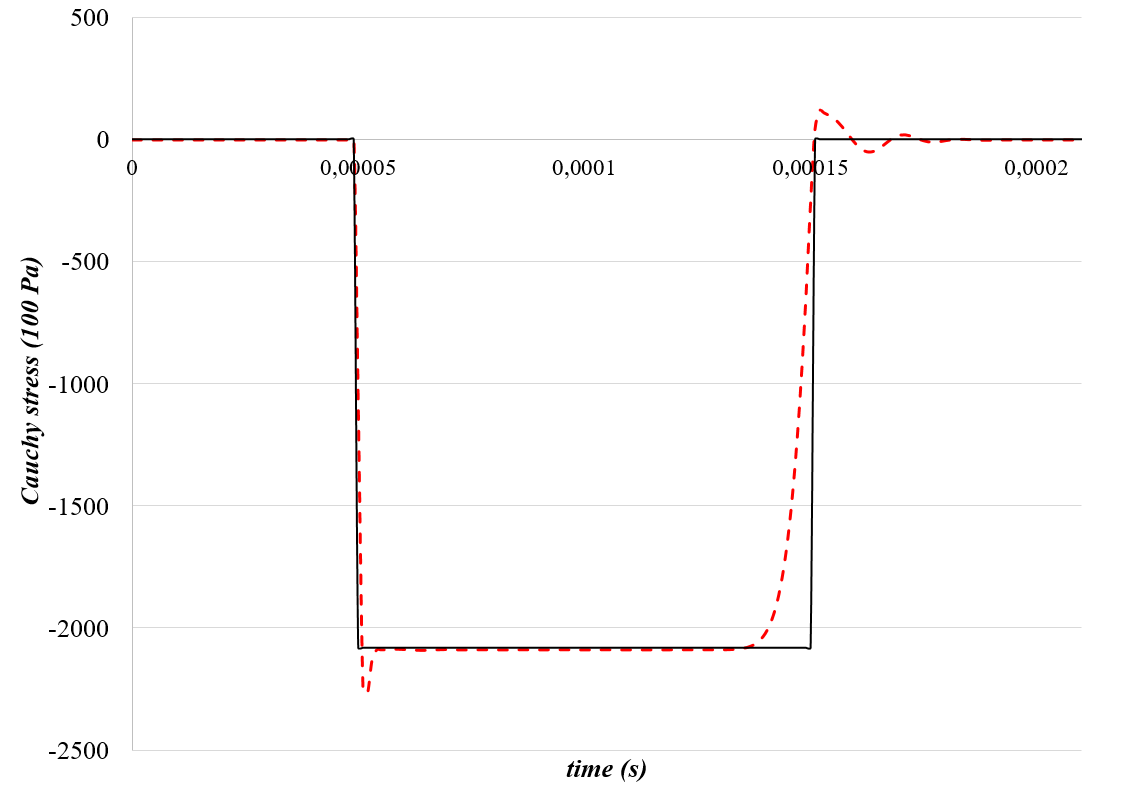
\includegraphics[scale=0.39]{Figures/contactVerification.png}
  \caption{Comparison between the analytical and numerical Cauchy stress $\sigma_{11}$ for the contact verification}
  \label{contactVerification}
  \end{center}
  \end{figure}

  Finally, we simulate the spreading, under gravity ($g = 9.81$ m/s$^2$), of a HBP fluid cube with an edge length of $0.1$ m containing $10\%$ immersed solid inclusions. The ground is modeled with solid elements to enable solid-solid interactions. The inclusions follow the Fuller curve distribution, with diameters from $0.020$ m to $0.030$ m, and both domains use a characteristic mesh length of $h_e = 0.0075$ m. The fluid has $\rho_f = 2200 \ \text{kg/m}^3$, $\tau_0 = 32.0$ Pa, $k = 255.0 \ \text{Pa·s}^n$, $0 = 1.0$, and $m = 1000.0$. The solids have $E = 1.0 \times 10^{11}$ Pa, $\nu = 0.0$, and $\rho_s = 2900 \ \text{kg/m}^3$. The nonlinear tolerance is $10^{-6}$, with $\Delta t = 0.01$ s and $1000$ time steps. Figure~\ref{megazorde}, although not a quantitative analysis, qualitatively confirms that the combined implementations of solid-solid and fluid-solid interactions are functioning as intended.
  \begin{figure}[!ht]
  \begin{center}
  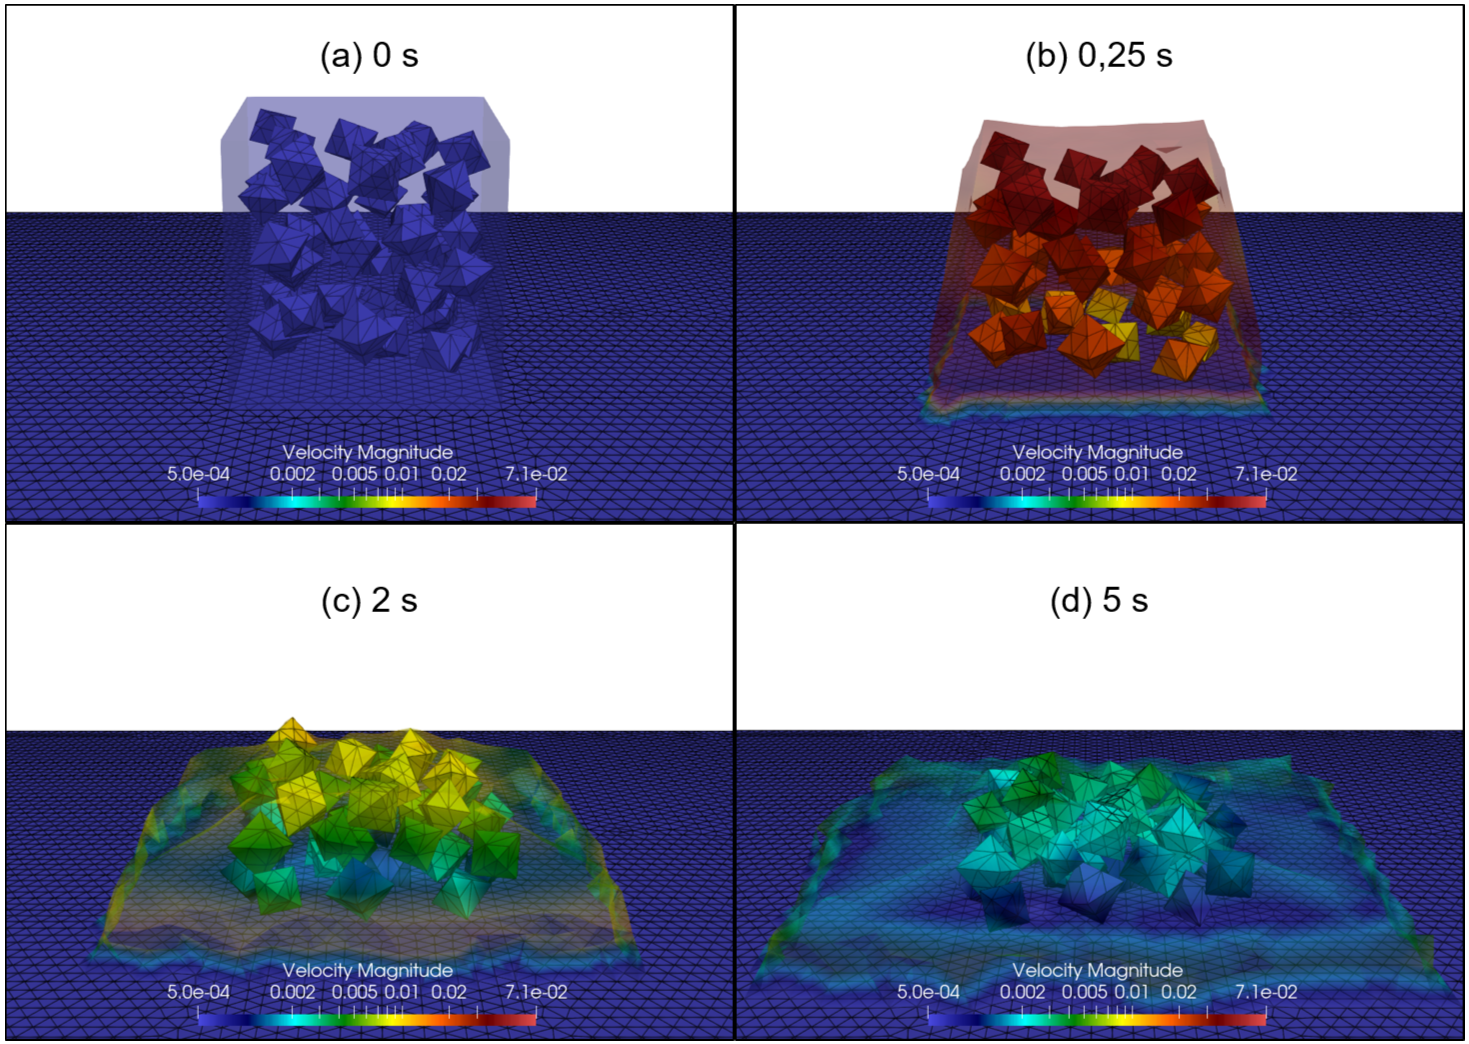
\includegraphics[scale=0.35]{Figures/megazorde.png}
  \caption{Simulation of combined solid-solid and fluid-solid interactions; units are in m/s}
  \label{megazorde}
  \end{center}
  \end{figure}
  % \vspace{8pt}

% --------------------------------------------------------------------------
\section{Conclusions}\label{sec:conclusion}
% --------------------------------------------------------------------------

  Separately, two benchmarks verified the correct implementation of the HBP constitutive model and the node-to-surface contact algorithm. By combining these two components with the monolithic fluid-solid coupling, the framework proposed in this work for simulating free-surface incompressible non-Newtonian flows with multiple immersed solid bodies shows strong potential for applications such as modeling concrete flow in the mesoscale, where the mortar is treated as a non-Newtonian fluid and the coarse aggregates as immersed elastic solid.

\vspace{20pt}
\noindent \textbf{Acknowledgements.} This study was financed in part by the Coordenação de Aperfeiçoamento de Pessoal de Nível Superior - Brasil (CAPES) - Finance Code 001, and by Brazilian National Council for Research and Technological Development (CNPq) - grant - 314045/2023-6. The authors would like to thank them for the financial support given to this research. The authors are also grateful for the infrastructure of the Department of Structures SET/EESC and the University of Sao Paulo.
\vspace{12pt}

%--------------------------------------------------------------------------
\noindent \textbf{Authorship statement.}
The authors hereby confirm that they are the sole liable persons responsible for the authorship of this work, and that all material that has been herein included as part of the present paper is either the property (and authorship) of the authors, or has the permission of the owners to be included here.


\bibliography{bibliography}

\end{document}